\documentclass[14pt]{extbook}
\usepackage{multicol, enumerate, enumitem, hyperref, color, soul, setspace, parskip, fancyhdr} %General Packages
\usepackage{amssymb, amsthm, amsmath, latexsym, units, mathtools} %Math Packages
\everymath{\displaystyle} %All math in Display Style
% Packages with additional options
\usepackage[headsep=0.5cm,headheight=12pt, left=1 in,right= 1 in,top= 1 in,bottom= 1 in]{geometry}
\usepackage[usenames,dvipsnames]{xcolor}
\usepackage{dashrule}  % Package to use the command below to create lines between items
\newcommand{\litem}[1]{\item#1\hspace*{-1cm}\rule{\textwidth}{0.4pt}}
\pagestyle{fancy}
\lhead{Makeup Progress Quiz 2}
\chead{}
\rhead{Version A}
\lfoot{2790-1423}
\cfoot{}
\rfoot{Summer C 2021}
\begin{document}

\begin{enumerate}
\litem{
Solve the linear equation below. Then, choose the interval that contains the solution.\[ \frac{3x + 7}{8} - \frac{-7x + 7}{5} = \frac{4x -7}{2} \]\begin{enumerate}[label=\Alph*.]
\item \( x \in [21.67, 26.67] \)
\item \( x \in [13.22, 15.22] \)
\item \( x \in [28.11, 33.11] \)
\item \( x \in [-2.5, 0.5] \)
\item \( \text{There are no real solutions.} \)

\end{enumerate} }
\litem{
Find the equation of the line described below. Write the linear equation in the form $ y=mx+b $ and choose the intervals that contain $m$ and $b$.\[ \text{Perpendicular to } 4 x - 7 y = 9 \text{ and passing through the point } (10, -5). \]\begin{enumerate}[label=\Alph*.]
\item \( m \in [-2.94, -1.6] \hspace*{3mm} b \in [11.5, 16.5] \)
\item \( m \in [-2.94, -1.6] \hspace*{3mm} b \in [-14.5, -9.5] \)
\item \( m \in [-2.94, -1.6] \hspace*{3mm} b \in [-18, -14] \)
\item \( m \in [-1.18, 0.03] \hspace*{3mm} b \in [11.5, 16.5] \)
\item \( m \in [1.29, 2.87] \hspace*{3mm} b \in [-23.5, -16.5] \)

\end{enumerate} }
\litem{
Write the equation of the line in the graph below in Standard Form $Ax+By=C$. Then, choose the intervals that contain $A, B, \text{ and } C$.
\begin{center}
    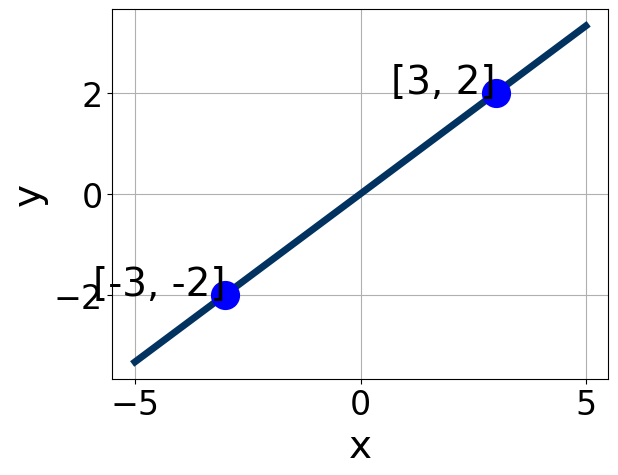
\includegraphics[width=0.5\textwidth]{../Figures/linearGraphToStandardCopyA.png}
\end{center}
\begin{enumerate}[label=\Alph*.]
\item \( A \in [1.4, 2.2], \hspace{3mm} B \in [2.31, 3.13], \text{ and } \hspace{3mm} C \in [0, 1] \)
\item \( A \in [-1.1, 1.8], \hspace{3mm} B \in [-2.36, -0.31], \text{ and } \hspace{3mm} C \in [0, 1] \)
\item \( A \in [1.4, 2.2], \hspace{3mm} B \in [-4.83, -2.98], \text{ and } \hspace{3mm} C \in [0, 1] \)
\item \( A \in [-1.1, 1.8], \hspace{3mm} B \in [0.09, 1.2], \text{ and } \hspace{3mm} C \in [0, 1] \)
\item \( A \in [-2.1, -1.8], \hspace{3mm} B \in [2.31, 3.13], \text{ and } \hspace{3mm} C \in [0, 1] \)

\end{enumerate} }
\litem{
First, find the equation of the line containing the two points below. Then, write the equation in the form $ y=mx+b $ and choose the intervals that contain $m$ and $b$.\[ (-6, 6) \text{ and } (-11, -10) \]\begin{enumerate}[label=\Alph*.]
\item \( m \in [0.2, 4.2] \hspace*{3mm} b \in [-27.2, -20.2] \)
\item \( m \in [0.2, 4.2] \hspace*{3mm} b \in [6, 16] \)
\item \( m \in [0.2, 4.2] \hspace*{3mm} b \in [1, 2] \)
\item \( m \in [0.2, 4.2] \hspace*{3mm} b \in [24.2, 27.2] \)
\item \( m \in [-3.2, -2.2] \hspace*{3mm} b \in [-48.2, -42.2] \)

\end{enumerate} }
\litem{
Solve the equation below. Then, choose the interval that contains the solution.\[ -17(-16x -18) = -7(-5x -9) \]\begin{enumerate}[label=\Alph*.]
\item \( x \in [-1.71, -1.38] \)
\item \( x \in [-1.38, -1.03] \)
\item \( x \in [-1.04, -0.79] \)
\item \( x \in [1.39, 1.7] \)
\item \( \text{There are no real solutions.} \)

\end{enumerate} }
\litem{
First, find the equation of the line containing the two points below. Then, write the equation in the form $ y=mx+b $ and choose the intervals that contain $m$ and $b$.\[ (9, -6) \text{ and } (-2, -2) \]\begin{enumerate}[label=\Alph*.]
\item \( m \in [-1.08, -0.24] \hspace*{3mm} b \in [-0.3, 0.13] \)
\item \( m \in [-1.08, -0.24] \hspace*{3mm} b \in [2.21, 3.36] \)
\item \( m \in [-0.18, 1.45] \hspace*{3mm} b \in [-1.84, -0.28] \)
\item \( m \in [-1.08, -0.24] \hspace*{3mm} b \in [-15.44, -14.63] \)
\item \( m \in [-1.08, -0.24] \hspace*{3mm} b \in [-2.91, -2.1] \)

\end{enumerate} }
\litem{
Solve the linear equation below. Then, choose the interval that contains the solution.\[ \frac{-3x + 8}{2} - \frac{-3x -3}{4} = \frac{-8x -4}{7} \]\begin{enumerate}[label=\Alph*.]
\item \( x \in [-9.73, -7.73] \)
\item \( x \in [-1.67, 1.33] \)
\item \( x \in [-39.18, -34.18] \)
\item \( x \in [-13.55, -10.55] \)
\item \( \text{There are no real solutions.} \)

\end{enumerate} }
\litem{
Find the equation of the line described below. Write the linear equation in the form $ y=mx+b $ and choose the intervals that contain $m$ and $b$.\[ \text{Perpendicular to } 5 x + 9 y = 9 \text{ and passing through the point } (2, 9). \]\begin{enumerate}[label=\Alph*.]
\item \( m \in [1.63, 2.26] \hspace*{3mm} b \in [-6.8, -4.4] \)
\item \( m \in [0.53, 0.7] \hspace*{3mm} b \in [2.5, 6.9] \)
\item \( m \in [1.63, 2.26] \hspace*{3mm} b \in [6.8, 7.5] \)
\item \( m \in [1.63, 2.26] \hspace*{3mm} b \in [2.5, 6.9] \)
\item \( m \in [-2.2, -1.18] \hspace*{3mm} b \in [11.5, 12.7] \)

\end{enumerate} }
\litem{
Write the equation of the line in the graph below in Standard Form $Ax+By=C$. Then, choose the intervals that contain $A, B, \text{ and } C$.
\begin{center}
    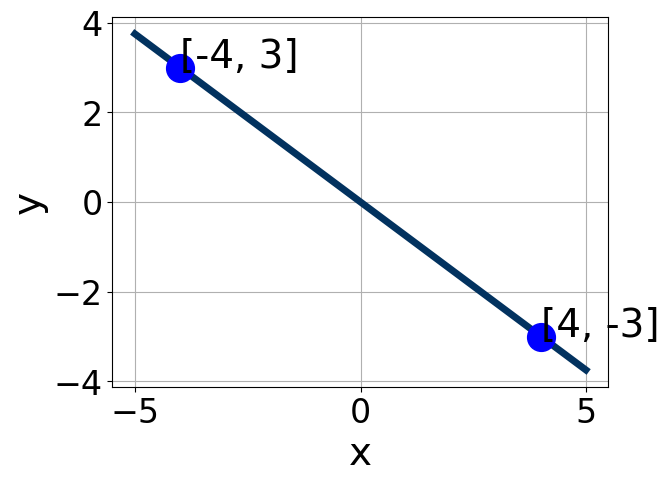
\includegraphics[width=0.5\textwidth]{../Figures/linearGraphToStandardA.png}
\end{center}
\begin{enumerate}[label=\Alph*.]
\item \( A \in [2.2, 4.6], \hspace{3mm} B \in [-5.6, -2.4], \text{ and } \hspace{3mm} C \in [0, 4] \)
\item \( A \in [0.3, 1], \hspace{3mm} B \in [-0.8, 1.4], \text{ and } \hspace{3mm} C \in [0, 4] \)
\item \( A \in [-5.2, -2.4], \hspace{3mm} B \in [-5.6, -2.4], \text{ and } \hspace{3mm} C \in [0, 4] \)
\item \( A \in [2.2, 4.6], \hspace{3mm} B \in [3.7, 4.6], \text{ and } \hspace{3mm} C \in [0, 4] \)
\item \( A \in [0.3, 1], \hspace{3mm} B \in [-2, -0.5], \text{ and } \hspace{3mm} C \in [0, 4] \)

\end{enumerate} }
\litem{
Solve the equation below. Then, choose the interval that contains the solution.\[ -10(-8x -4) = -15(6x -12) \]\begin{enumerate}[label=\Alph*.]
\item \( x \in [-1.68, -0.73] \)
\item \( x \in [0.72, 1.17] \)
\item \( x \in [1.2, 1.78] \)
\item \( x \in [21.99, 22.46] \)
\item \( \text{There are no real solutions.} \)

\end{enumerate} }
\end{enumerate}

\end{document}